\documentclass[10pt]{nsibeamer}
\title{Chapitre 05 : Bases de données}
\subtitle{Partie 4}
\author{NSI2}

\setminted{fontsize=\footnotesize}
\setmintedinline{fontsize=\normalsize}

\begin{document}
	\maketitle
    \section{Requêtes SQL}
\begin{frame}{Requête et résultat}
Une requête est une commande SQL et renvoie une table.\\
On se replace dans le contexte du chapitre précédent.
\end{frame}
\begin{frame}[fragile]{Sélection d'attributs}
	\begin{minted}{sql}
SELECT nom, prenom
FROM Auteur;
    \end{minted}
    \pause
    \begin{center}
    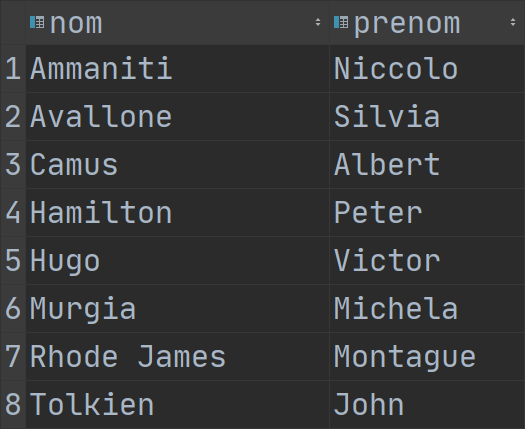
\includegraphics[height=6cm]{img/requete 1}
    \end{center}
\end{frame}

\begin{frame}[fragile]{Sélection de tous les attributs}
	\begin{minted}{sql}
SELECT *
FROM Auteur;
    \end{minted}
    \pause
    \begin{center}
    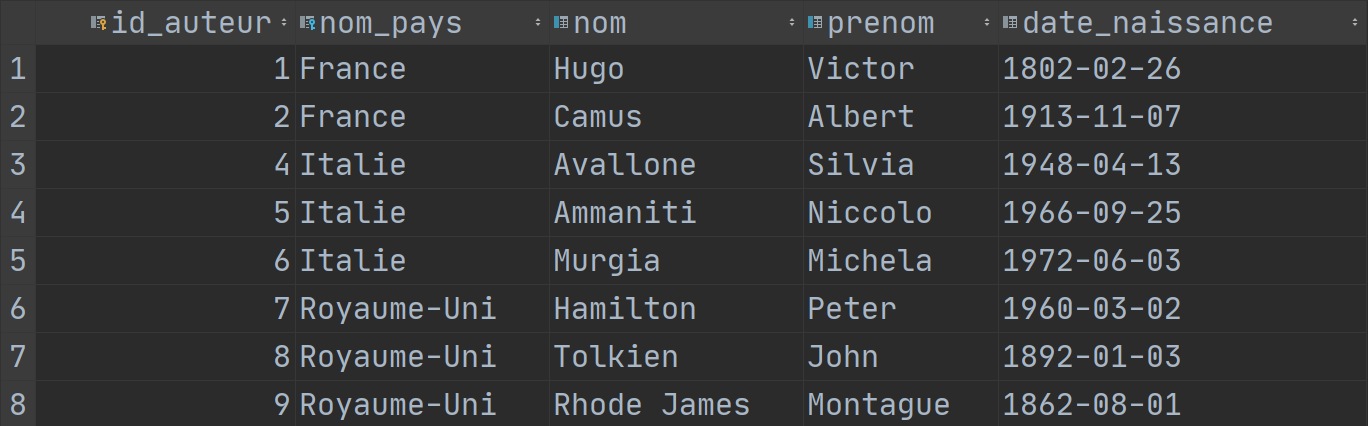
\includegraphics[width=11cm]{img/requete 2}
    \end{center}
\end{frame}

\begin{frame}[fragile]{Sélection avec condition}
	\begin{minted}{sql}
SELECT nom, date_naissance
FROM Auteur
WHERE date(date_naissance) < '1900';
    \end{minted}
    \pause
    \begin{center}
    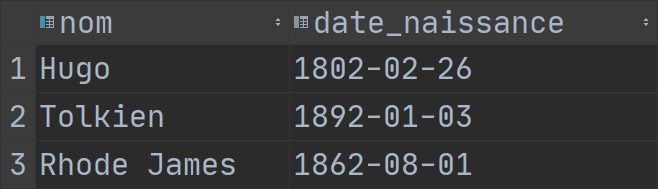
\includegraphics[width=8cm]{img/requete 3}
    \end{center}
\end{frame}

\begin{frame}[fragile]{Sélection avec conditions multiples}
	\begin{minted}{sql}
SELECT nom, date_naissance
FROM Auteur
WHERE date(date_naissance) < '1900'
  AND nom_pays = 'France';
    \end{minted}
    \pause
    \begin{center}
    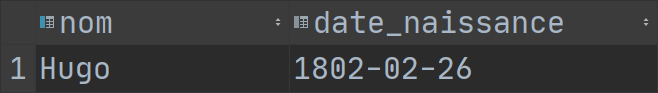
\includegraphics[width=8cm]{img/requete 4}
    \end{center}
\end{frame}

\begin{frame}[fragile]{Renommer les colonnes}
	\begin{minted}{sql}
SELECT titre AS Titre_ouvrage, num_isbn AS Reference_ISBN
FROM Livre
WHERE date(annee) > '2015';
    \end{minted}
    \pause
    \begin{center}
    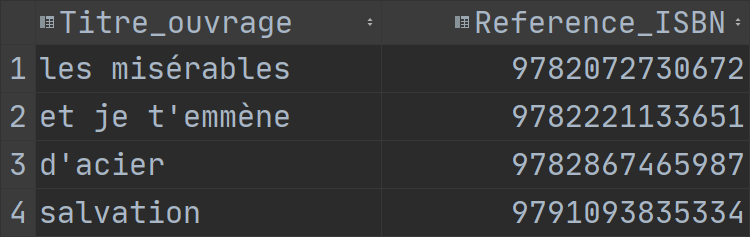
\includegraphics[width=8cm]{img/requete 5}
    \end{center}
\end{frame}

\begin{frame}[fragile]{Fonction COUNT}
	\begin{minted}{sql}
SELECT COUNT(titre) AS Nb_Livres_avant_2015
FROM Livre
WHERE annee < 2015;    \end{minted}
\pause
    \begin{center}
    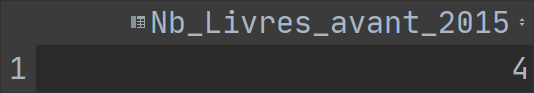
\includegraphics[width=8cm]{img/requete 6}
    \end{center}
\end{frame}
\begin{frame}{Autres fonctions similaires}
	Fonctions MIN, MAX, SUM et AVG (moyenne).
\end{frame}
\begin{frame}[fragile]{\'Eliminer les doublons}
Sans élimination :
	\begin{minted}{sql}
SELECT id_auteur
FROM Ecrire;
    \end{minted}
    \pause
    \begin{center}
    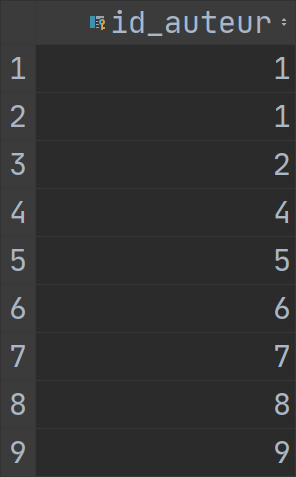
\includegraphics[width=3cm]{img/requete 7}
    \end{center}
\end{frame}

\begin{frame}[fragile]{\'Eliminer les doublons}
Avec élimination :
	\begin{minted}{sql}
SELECT DISTINCT id_auteur
FROM Ecrire;
    \end{minted}
    \pause
    \begin{center}
    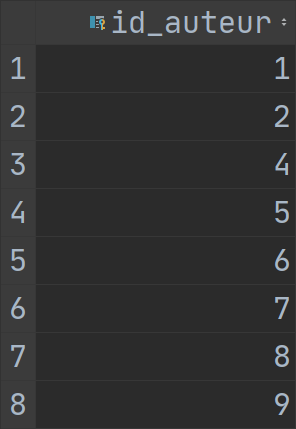
\includegraphics[width=3cm]{img/requete 8}
    \end{center}
\end{frame}

\begin{frame}[fragile]{Ordonner les tuples}
Ordonner les noms dans l'ordre croissant :
	\begin{minted}{sql}
SELECT nom,prenom FROM Auteur
ORDER BY nom ASC;
    \end{minted}
    \pause
    \begin{center}
    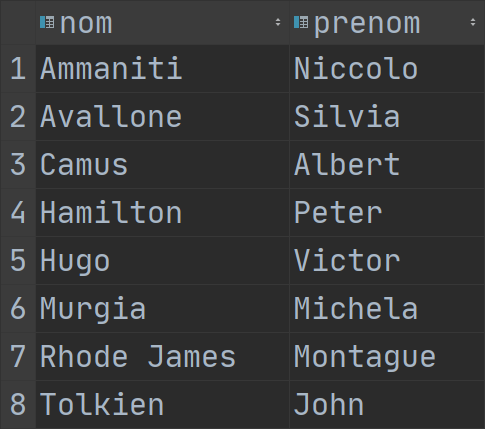
\includegraphics[width=3cm]{img/requete 9}
    \end{center}\pause
    Pour l'ordre décroissant on utilise \mintinline{sql}{DESC}.
\end{frame}

\section{Jointures}
\begin{frame}{Principe}
	Considérons 2 tables T1 et T2 et supposons que c est une clé étrangère qui fait référence à b.\pause
    \begin{center}
        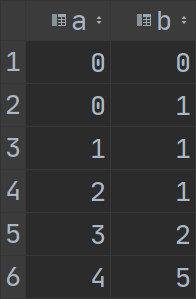
\includegraphics[width=3cm]{img/j1}\ \ 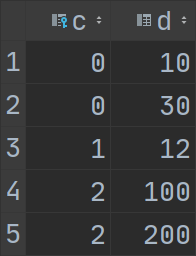
\includegraphics[width=3cm]{img/j2}
        \end{center}\pause
    Voici table qui est la \alert{jointure} T1 et T2 selon la condition b=c :
\end{frame}

\begin{frame}{Principe}
    \begin{center}
        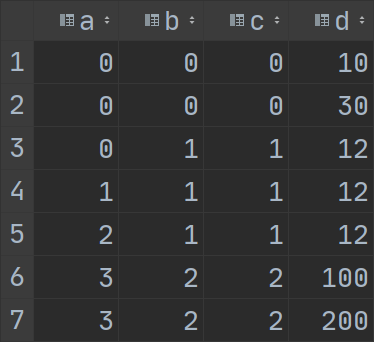
\includegraphics[width=6.3cm]{img/j3}
        \end{center}\pause
       C'est la table obtenue en faisant correspondre chaque tuple de T1 avec chaque autre tuple de T2 tel que b et c soient égaux.
\end{frame}
\begin{frame}[fragile]{Applications}
	Produire la table des noms des auteurs venant de pays de plus de 61 millions d'habitants :\pause
    \begin{minted}{sql}
SELECT nom
from Auteur
         JOIN Pays ON Auteur.nom_pays = Pays.nom_pays
WHERE population > 62000000;
    \end{minted}
    \pause
     \begin{center}
            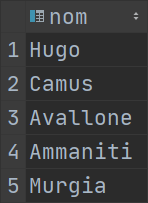
\includegraphics[width=3cm]{img/requete 10}
     \end{center}
\end{frame}



\begin{frame}[fragile]{Applications}
	Produire la table des noms et prénoms des auteurs ayant écrit un livre dont le titre comporte « la»  :\pause
\begin{minted}{sql}
SELECT DISTINCT nom, prenom
FROM Auteur
         JOIN Ecrire ON Ecrire.id_auteur = Auteur.id_auteur
         JOIN Livre ON Livre.num_isbn = Ecrire.num_isbn
WHERE Livre.titre LIKE '%la%';
\end{minted}
\pause
     \begin{center}
            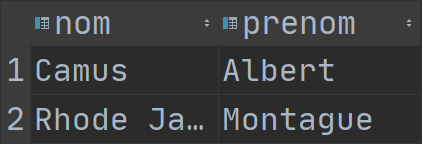
\includegraphics[width=5cm]{img/requete 11}
     \end{center}
\end{frame}
\section{Mises à jour}


\begin{frame}[fragile]{INSERT INTO}
Insérer un nouveau tuple dans la table \textbf{Auteur} :\pause
\begin{minted}{sql}
INSERT INTO Auteur VALUES
    (128,'France','Leleu','Frédéric','1974-05-16');
\end{minted}
\pause
Les colonnes doivent être dans le même ordre qu'à la création, sinon utiliser\pause
\begin{minted}{sql}
INSERT INTO Auteur VALUES (nom,id_auteur)
    ('Leleu',128);
\end{minted}
\pause
Les colonnes non renseignées prendront par défaut la valeur \mintinline{sql}{NULL} ce qui peut poser problème.
\end{frame}

\begin{frame}[fragile]{DELETE}

Supprimer les tuples de \textbf{Ecrire} dont l'auteur a l'id\_auteur 1:\pause
\begin{minted}{sql}
DELETE FROM Ecrire WHERE id_auteur = 1;
\end{minted}
\pause
Penser aux contraintes de références (clé étrangères) : si on supprime un tuple et qu'un tuple d'une autre table fait référence à celui qu'on supprime, cela provoquera une erreur.
\end{frame}

\begin{frame}[fragile]{UPDATE}

	Mettre à jour l'id du tuple de \textbf{Auteur} dont le nom est Hugo\pause
	\begin{minted}{sql}
UPDATE Auteur
SET id_auteur = 1024
WHERE nom = 'Hugo';
	\end{minted}
    \pause
Penser aux contraintes de références (clé étrangères) lors de la mise à jour.
\end{frame}
\end{document}